\citep{Blomstrom2002}

\subsubsection{The model of interaction between the local and central governments}

The game has two players: the central government and the provincial official. The sequencing of the game is as follows:
\begin{enumerate}
\item At the start of the game, the endowment of a province is given.\footnote{The assumption that the endowment is exogenous is reasonable. First, if it is the kind of endowment that cannot be affected by past provincial policies, e.g. natural resources, proximity to market, then it is truly exogenous. Second, even if it is the kind of endowment that can be affected by past policies, e.g. quality of the labor force, infrastructure quality, etc., it is usually good for both foreign and domestic firms. Therefore, at the start of the game, there is not yet any discrimination between foreign and domestic firms.}
\item The provincial official observes his endowment and calculates his current wealth, i.e. the bribes from FDI firms that chose his province due to its endowment.
\item The provincial official calculates the return of pursuing a promotion, which is a ``gamble'' with uncertainty. In this gamble,

the return of pursuing a promotion $=$ the return of the promotion $\times$ the probability of getting the promotion $(p)$.

In addition, $p = p_0 + p_1$, with $p_0$ being the base chance of getting the promotion, and $p_1$ being the added chance if the official decides to develop the domestic sector as the central government desires.

\item The provincial official has to decide between keeping his current wealth (i.e. seek rents from FDI) or gambling (i.e. focus on private sector development to get a $p_0 + p_1$ chance of getting the promotion). Assuming that the official is risk averse, he prefers a small gamble over a large one. In this way, the base chance $p_0$ matters. If $p_0$ is small, it is highly uncertain that the official will get the promotion even with the added $p_1$. Therefore, the official is more likely to seek rent from the foreign firm instead of pursuing a promotion when the base chance $p_0$ is small. 
\end{enumerate}

\item Is it reasonable to frame seeking rents and seeking technological spillover from FDI as a dichotomous choice for provincial officials?

In the above model, provincial officials have to choose between attracting FDI for spillover or for bribes. One may argue that this trade off does not exist. Indeed, if the fact that a foreign firm engages in corruption does not affect its level of spillover, then even if provincial officials prioritize FDI for rents it would not have any effect on the level of spillover.

However, the trade off does exist. This is because, in exchange for bribes, provincial officials must offer some advantages over domestic firms to foreign firms. This can be lower tax rate, easier access to land, more attention to concerns of firms, etc. Without efforts by the local government to nurture the private sector, it is unlikely that private firms have the necessary sophistication to engage in contracts with foreign firms or to imitate foreign firms' technology.

\Cref{fig:fdi_bias_vietnam} provides evidence that when provincial officials are biased towards foreign firms, private firms are poorly supported. The x-axis shows how helpful the province is according to private firms. The y-axis shows the fairness of provincial officials in treating foreign and private firms (as perceived by private firms). The graph shows that if a province is biased towards foreign firms, it will also treat private firms poorly (the lower-left quadrant). The relationship is even stronger among provinces with a lot of FDI (blue labels and line).
\end{enumerate}

\begin{figure}[!ht]
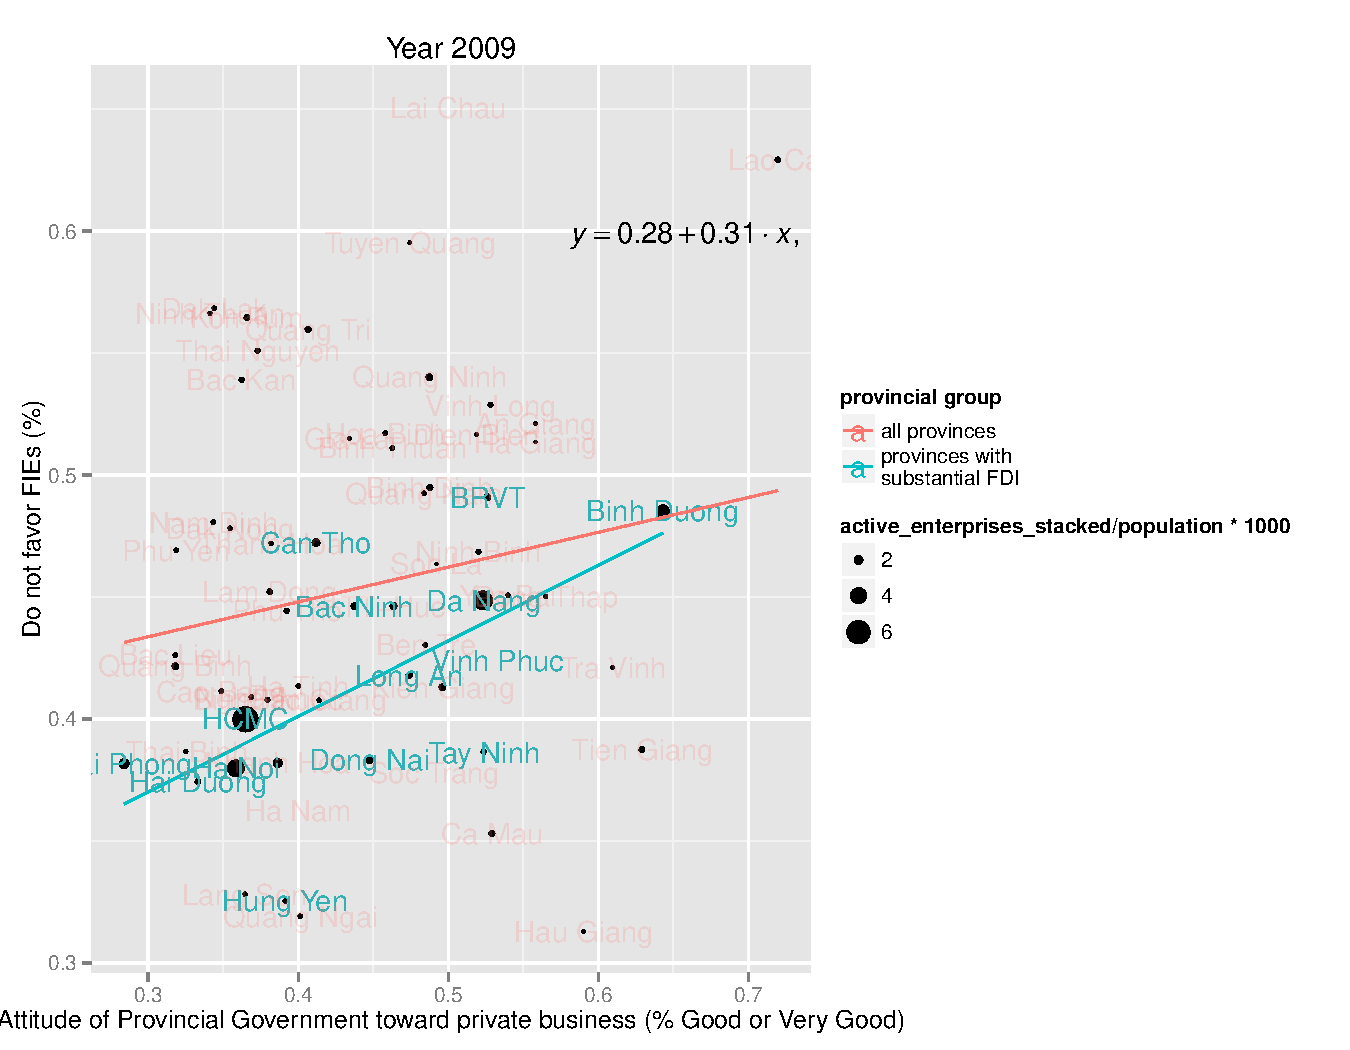
\includegraphics[width=\textwidth,keepaspectratio]{../figure/FDI_bias}
\caption{The relationship between a province's FDI bias and attitude towards the private sector}
\label{fig:fdi_bias_vietnam}
\end{figure}

As well-known from neoclassical growth theory, the diminishing return to capital will at one point stop capital from accumulating further, preventing long-run economic growth to be permanently driven by capital accumulation alone \citep{Solow1956}. Therefore, long-run growth ultimately requires technological innovation, which continually increases the productivity of capital and counteracts the diminishing returns.

This insight implies that FDI cannot promote the host country's growth simply from the amount of capital it brings. Therefore, FDI only has a highly uncertain impact on growth and poverty reduction \citep{Nair-Reichert2001, Carkovic2002, Guerra2009}. Scholars have further confirmed that FDI can only a growth-enhancing impact if there is technological spillover from the foreign to the domestic sectors \citep{Nunnenkamp2004}. This empirical finding provides support for \citet{Findlay1978}'s groundbreaking model of FDI and growth, in which technology spillover from foreign firms shift the domestic factor-price frontier to the right, allowing more output from the same input, resulting in higher profits and higher wages (i.e. higher savings) for the domestic sector. This ultimately leads to a continually increasing domestic capital stock.

Since FDI can only be beneficial to growth if there is technological spillover, if one does not observe spillover, it must mean that the host government is attracting FDI for reasons other than growth. In the next step in the theory, I argue that bribe from foreign firms is one such reason.

\subsection{Defining corruption}

Defining corruption has been a long-standing and inconclusive debate \citep{Johnston1996}. The contention stems from the normative nature of the ``corruption'' concept, which shifts significantly across context and thus difficult to build an analytical edifice upon. 

Consider the most common definition of corruption as ``the abuse of public roles for private gains.'' Make no mistake, this definition is not always clear cut. What constitutes ``abuse''? The term implies the violation of certain standards, which only further asks: what standards are supposed to be adhered to? Some scholars emphasize law-based standards, but the law is not always legitimate \citep[17]{Johnston2004}. Yet others argue for norm-based standards, but difference in norms across societies can be so extensive and unsystematic that renders a cross-country analysis untenable. Indeed, nepotism and cronyism in one society may be social capital in another, with all shades of favoritism in between \citep{Rosen2010}. 

In addition, the distinction between ``public'' and ``private'' are not always clear, especially during rapid economic liberalization and privatization. As the rules change continuously, the dividing line between an innovator and a rule-breaker is but a thread left blowing in the political wind \citep{Sun2004}.

In spite of its shortcomings, the definition of corruption as the ``abuse of public role for private gains'' works well for my research. While this definition may fail as a universal classification of corrupt act, within the scope of my research project its unclarities are largely resolved. First, regarding the unclarity over ``abuse,'' I focus on a law-based definition because of its precision, stability, and broad coverage. The legitimacy of the ``law'' is not as big of a concern because the vast majority of countries with substantial FDI maintain sovereignty over their territory and have laws with a binding impact on their economic life, especially the formal sector in which foreign firms operate. (List the countries in the doing business survey, and whether any of them is a failed state). In addition, a law-based definition fits well with the way corruption is often framed in business surveys, my main source of data, as ``paying informal fees.'' Regardless of whether the respondents think these fees are legitimate or acceptable, it is clear to both the officials and the firms whether these fees are official, as documented in formal laws.

Second, the ``public'' and ``private'' divide is also clear cut within the scope of my project. I focus on corrupt acts in the context of officials exchanging public resources under their control for bribes from foreign firms (e.g., expedited bureaucracy, access to land, harass-free inspections, etc.). It is clear that these public resources and services should be distributed fairly, and that the payments are going to the officials' private wealth instead of the state's coffer.

\subsection{Anticipating counter arguments}

There are several reasons why the government is interested in seeking rent from FDI firms instead of domestic firms. First, if foreign firms are more profitable than domestic firms, they have more rent to be extracted. Second, if foreign firms are larger than domestic firms, they facilitate coordination and allow corruption to be better kept secret among fewer actors. Third, if the interests of firms and the government misalign in the future, foreign firms have both the options of ``exit'' and ``voice,'' whereas domestic firms only have ``voice.'' The government would much prefer an exiting foreign firm to a domestic firm voicing its interest. The first and second reasons also indicate that my theory is most applicable when the entering FDI firms are large.